% Created 2024-11-22 fre 12:55
% Intended LaTeX compiler: xelatex
\documentclass[a4paper, 12pt]{article}
\usepackage{graphicx}
\usepackage{longtable}
\usepackage{wrapfig}
\usepackage{rotating}
\usepackage[normalem]{ulem}
\usepackage{amsmath}
\usepackage{amssymb}
\usepackage{capt-of}
\usepackage{hyperref}
\usepackage[danish]{babel}
\usepackage[top=2.0cm,bottom=2.0cm,hmargin=3.0cm]{geometry}
\usepackage{hyperref}
\hypersetup{colorlinks, linkcolor=black, urlcolor=blue}
\setlength{\parindent}{0em}
\parskip 1.5ex
\author{Jacob Debel}
\date{Fysik B}
\title{Mekanik\\\medskip
\large Simple opgaver om translatorisk kinematik}
\hypersetup{
 pdfauthor={Jacob Debel},
 pdftitle={Mekanik},
 pdfkeywords={},
 pdfsubject={},
 pdfcreator={Emacs 29.4 (Org mode 9.6.15)}, 
 pdflang={Danish}}
\begin{document}

\maketitle


\section*{Bevægelse med konstant hastighed}
\label{sec:org9d3f065}

\subsection*{Opgave 1}
\label{sec:orgbe1d601}

En cyklist kører med konstant hastighed strækningen 35 km på 2 timer og 10 min.

\begin{enumerate}
\item Find cyklistens hastighed både i m/s og km/h.

\item Hvor langt er cyklisten nået efter 35 min.?
\end{enumerate}

\subsection*{Opgave 2}
\label{sec:org71456f1}

Et tog kører med konstant hastighed. Figur \ref{tog} viser togets position som funktion af tiden.
\begin{figure}[htbp]
\centering
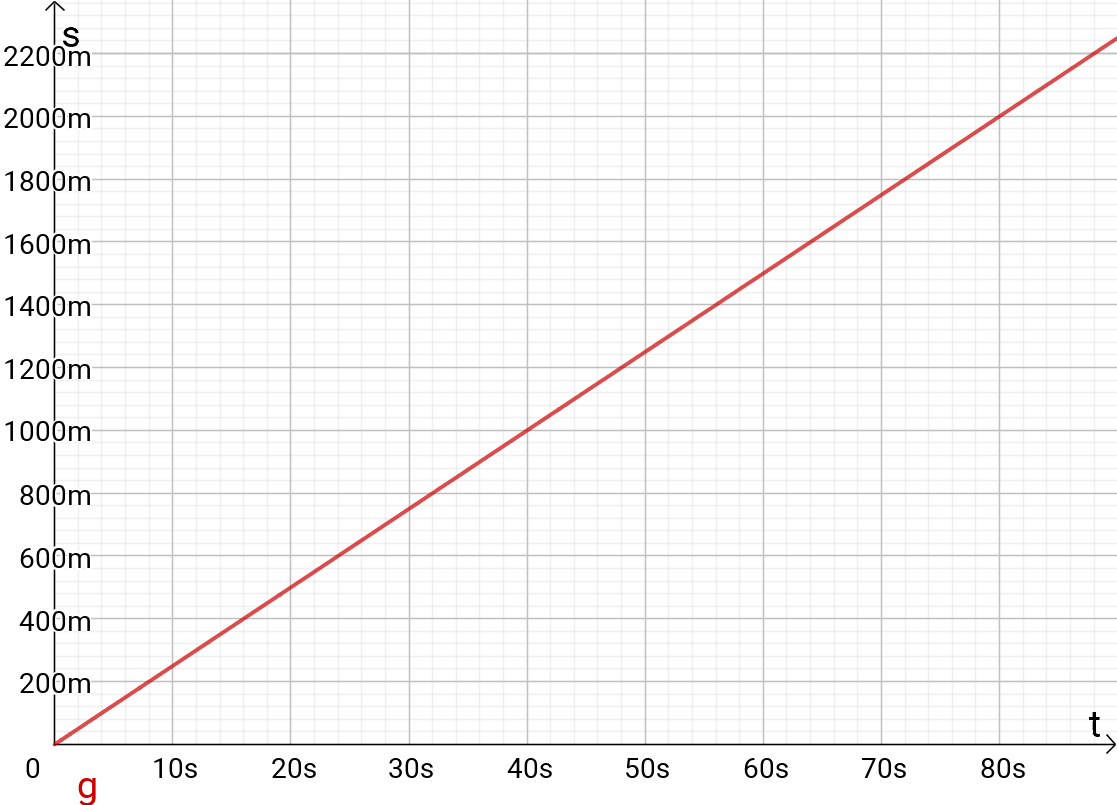
\includegraphics[width=0.6\linewidth]{img/tog.png}
\caption{\label{tog}(t,s)-graf for togets bevægelse.}
\end{figure}

\begin{enumerate}
\item Bestem togets hastighed ud fra grafen.

\item Omregn togets hastighed til km/h.
\end{enumerate}

\section*{Bevægelse med konstant acceleration}
\label{sec:org20abcae}

\subsection*{Opgave 3}
\label{sec:org44fbfed}

En bold kastes lodret op i luften med en fart på 20 m/s.

\begin{enumerate}
\item Indlæg en koordinatakse og angiv accelerationen i forhold til denne.

\item Hvor højt op når bolden?

\item Bestem \textbf{stigetiden} og siden \textbf{faldtiden} tilbage til udgangspunktet.
\end{enumerate}

\subsection*{Opgave 4}
\label{sec:org9486c67}

Det siges i teoribøgerne til køreundervisning, at en fordobling af farten medfører en firedobling af bremselængden.

Ved at blokere bremserne bruger en bil 23 m til at foretage en opbremsning fra 70 km/h.

\begin{enumerate}
\item Beregn bilens maksimale accelerationsevne (decelerationsevne) ved opbremsning.

\item Beregn bremselængden, når bilen kører med 140 km/h.

\item Hvor stærkt skal bilen køre, for at bremselængden bliver fordoblet til netop 46 m?
\end{enumerate}

\subsection*{Opgave 5}
\label{sec:org26ea9db}

En bil og en cykel starter fra samme udgangspunkt. Cyklisten accelererer op til 46 km/h med en acceleration på 2.0 \(m/s^2\), hvorefter den opnåede hastighed fastholdes. Bilen accelererer med en konstant acceleration på 1.0 \(m/s^2\).

\begin{enumerate}
\item Indtegn (t,v)-graferne for bilen og cyklen i det samme koordinatystem.

Benyt geogebra til dette.

\item Bestem det tidspunkt samt hvor langt fra udgangspunktet at cykel og bil er ud for hinanden igen.
\end{enumerate}

\section*{Vilkårlig bevægelse}
\label{sec:org0a95869}

\subsection*{Opgave 6}
\label{sec:org798fe1d}

\begin{center}
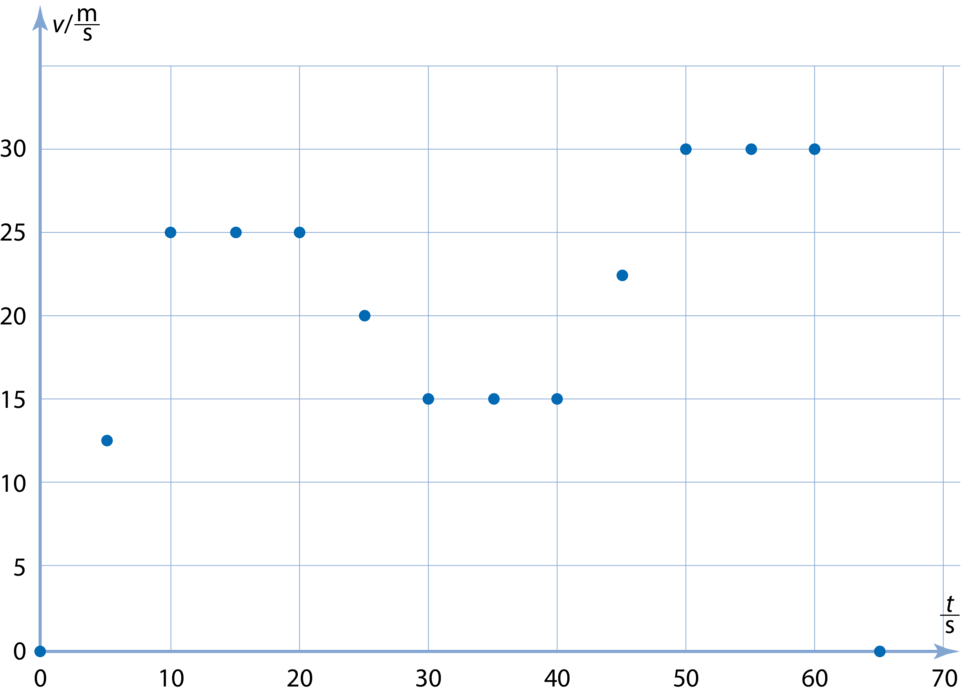
\includegraphics[width=10cm]{img/2019-11-05_08-08-27_csm_76_Maalte_hastigheder_01_5964e15f5a.png}
\end{center}

Grafen viser 14 målinger af hastigheden for forskellige tidspunkter.

\begin{enumerate}
\item Beskriv bevægelsen ud fra de kinematiske begreber og grafen.
\item Hvor sker der acceleration, og hver er der konstant hastighed?
\item Bestem accelerationen i de forskellige intervaller.
\item Find den samlede tilbagelagte strækning fra 0 s til 65 s.
\end{enumerate}

\subsection*{Opgave 7}
\label{sec:org2949c68}

\begin{itemize}
\item Skitsér en (t,s)-graf, som viser en bil, hvor positionen vokser, mens hastigheden aftager.

\item Skitsér en graf, hvor positionerne er negative, mens hastigheden er positiv.

\item Skitsér en graf, hvor positionerne er negative, og hastigheden også er negativ.

\item Skitsér en graf, hvor positionerne er voksende, mens hastigheden er negativ.
\end{itemize}
\end{document}
